\documentclass[a4paper]{article}
\usepackage{amsmath,amsfonts}
\usepackage{graphicx}
\usepackage{hyperref}


% setup font
\usepackage[sc]{mathpazo}
\linespread{1.05}
\usepackage[T1]{fontenc}

\usepackage{todo}

\author{Boris Reuderink\\\texttt{boris@cortext.nl}}
\title{Analysis plan for AlgorithmWatch TAMI Dutch politics data}

\begin{document}
\maketitle
\tableofcontents
\section{Introduction}
Towards a Monitoring of Instagram (TAMI) is a controlled experiment that will
shed light on how items are chosen by Instagram's algorithm, focusing on
political parties in the Netherlands. The results will be shared with NRC to
produce a series of articles. Then project will be successful when Instagram
users in the Netherlands know more about our findings (measured by engagement
on NRC and their Instagram feed) and if Instagram reacts meaningfully to our
findings.

\subsection{Aims}
The aim of the data analysis is to reveal if specific types of posts on
Instagram are overrepresented (i.e. are relatively more likely to show up in
a users feed). We distinguish between two types of overrepresentation: 1)
overrepresentation driven by post popularity, such as for viral content, and
2) overrepresentation driven by biases in Instagram’s recommendations. We are
particularly interested in the latter type of overrepresentation. Note that
this biased overrepresentation might differ from user to user. With the
analysis described below, we collect evidence to answer the following
research questions:

\label{sec:RQ}
\paragraph{RQ1: What posts are overrepresented in the encounters?}
To answer this question, we need to describe what posts of Dutch politicians on
Instagram are overrepresented in general. This might be due to popularity of
the post, or due to biases in Instagram’s recommendations. We are interested
in topics, as indicated by hashtags and by GoogleVision results for the
post's images.

\paragraph{RQ2: What posts are overrepresented given their
popularity?} Since overrepresentation is likely to driven by popularity, we
analyse what types of posts are overrepresented if we correct for effects of
post popularity. Remaining variations in post popularity can indicate biases
in Instagram’s recommendations.

\paragraph{RQ3: Is the overrepresentation the same in all subgroups?}
There might be biases that promote user engagement, such as bias for
controversial content. But we might also find biases due to personalization.
Biases due to personalization are expected to vary from user to user, while
consistent biases are present for all users. We test the consistency of
biases by evaluating the predictive performance of bias models on users that
were not used for model development.

\paragraph{RQ4: Who benefit from these discrepancies?}
Finally, we can estimate per politician how much their posts were benefitting
from a consistent algorithm bias of Instagram's recommendations.


\subsection{Data generation}
The data from the TAMI experiment was generated as follows. A list with
accounts from Dutch politicians was used to monitor all posts by these
accounts in a certain period. A group of voluntary data donors ran a
browser-plug that retrieved the top posts in the timeline at hourly
intervals, and records if a post from the monitored accounts was encountered.
Donors were asked to follow a particular set of of three politicians. 

We have no information on the exact ranking algorithm that Instagram uses to
determine what posts to present in the timeline of a user. Based on general
properties of recommendation systems we expect that a the probability of
encountering a posts is based on: the popularity of the post, the time of
day, and day of week, the content of the post, and content preferences of the
user. A graph of the assumed data generating processes is shown in
Figure~\ref{fig:data_generation}. 

\begin{figure}
    \centering
    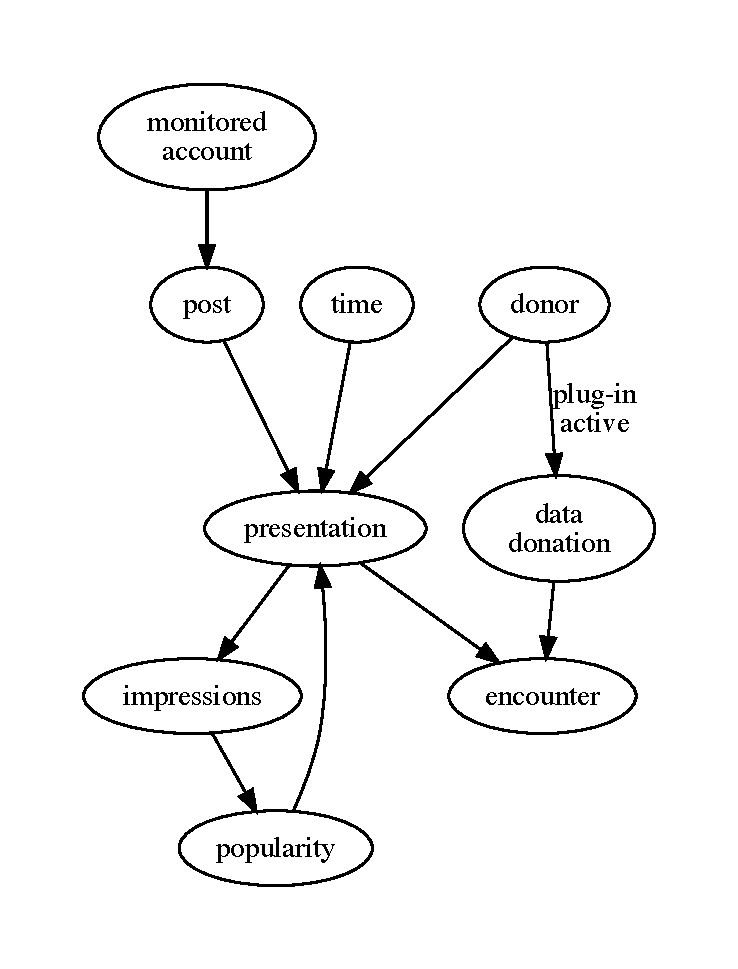
\includegraphics[width=0.5\textwidth]{data_generation.pdf}
    \caption{Schematic overview of the data generating process. Note that
    there is a feedback loop where increased impressions lead to increased
    popularity, which in turn leads to increased presentation of a post.}
    \label{fig:data_generation}
\end{figure}

\section{Analysis}
First we pre-process data using database queries into a representation that
facilitates easy analysis. We select time periods where a donor could have
observed a particular post, and model the probability of an encounter in this
period by fitting a logistic regression model. Properties of this models can
answer RQ1. Next, we add features (exogenous variables) for post popularity.
Properties of this model can answer RQ2. To evaluate the consistency of the
found biases, we evaluate the properties of the found model on held-out
donors. Due to the small number of donors we use cross-validation, where the
procedure is repeated for different sets of held-out donors. Finally, we make
take the consistent effects to estimate the expected algorithm bias per
account, and per political party (RQ4).

\subsection{Preprocessing}
We organize the analysis around potential encounters of posts of monitored
politicians by donors at hourly intervals. Only the first 7 days after
post-creation are considered. For each of potential encounter, we store the
following dynamic properties at hourly intervals: the number of likes, the
number of comments, and the presence of an encounter. This data is stored in
a table~$T_d$.

We use information from posts to model the probability of an encounter given
a certain post. To this end, we prepare a representation of posts with
properties that can explain the probability of an encounter. It is based on
results from the Google Vision API (safe search, label annotations), hashtags
from the post text, and the number of followers of the politician's account.
This static data is stored in table~$T_s$.

\subsection{Modeling}
In the previous section we introduced the tables with data that does not vary
with time ($T_s$) and with data that does vary with time ($T_d$). In this
section we outline a series of analysis steps that will lead to evidence to
answer the research questions introduced in section~\ref{sec:RQ}.

\subsubsection{Post overrepresentation} \label{sec:overrep}
% Describe steps to model popularity as function of post properties (describe properties) for RQ1.
RQ1 is about what types of posts are overrepresented in general. Since we
organized our data around potential encounters, we can use the static
properties from $T_s$ to predict the presence of an encounter in the time
window with a logistic-regression model. In addition, we include a donor ID
in the predictors to automatically account for difference in the amount of
posts from other followed accounts. Coefficients of this regression model
indicate how different post properties contribute to overrepresentation.
Alternatively, we can use feature permutation to quantify how much a specific
post property contributes to predictive performance.

\subsubsection{Bias} \label{sec:bias}
% Describe steps to model encounter probability based on post type controlling for popularity for RQ2.
For RQ2 we need to know what types of post are overrepresented given their
popularity. We add information on post popularity and repeat the analysis in
section~\ref{sec:overrep}.

\subsubsection{Consistency of bias}
% Describe steps to model encounter probability based on post type
% controlling for popularity and subgroup for RQ3.
Effects of overrepresentation found while controlling for post popularity
indicate a bias of Instagram's recommendations. This bias might be
consistent, but it might also be a consequence of personalization. To find
consistent biases, we evaluate how much individual post properties contribute
to predicting encounters on held-out donors. If a post property consistently
contributes to accurate predictions of engagements for other donors we have
found a consistent bias. This is quantified using permutation feature
importance on held-out data.

Due to the low-number of donors, we have to train multiple models, where
different donors are used as held-out data. For each of these models, we have
to perform the analysis, and combine the results to construct a final
set of biases.

\subsubsection{Interpreting bias at account and party level}
% Describe how to connect the results to individual accounts and political parties.
Finally, the biases found in section~\ref{sec:bias} can be estimated on the
user account level, and aggregated on the political party level. This can be
done by setting the models coefficients for popularity features to zero, 
making a prediction, and performing the aggregation. 

\todos
\end{document}
